\documentclass{beamer}
\usetheme{Madrid}
\usepackage[italian]{babel}

\title[Trading AI]{Progettazione e sviluppo di test suite automatica e modulo raccolta dati per intelligenze artificiali che si occupano di creare strategie di investimento}
\author{Garion Musetta}
\centering
\date{Aprile 2020}
\begin{document}
\maketitle

\begin{frame}{Contesto}
\begin{itemize}
\item Nexid Edge blockchain e AI sviluppa strumenti intelligenti per l’analisi del mercato delle criptovalute e
la creazione di strategie di investimento
\item Realizza Smart Contract sulla Blockchain Ethereum per la certificazione di opere in vari settori
\item Ha creato Sentyment AI, strumento in grado di prevedere il mercato finanziario delle criptovalute e di creare \textbf{strategie di investimento} intelligenti
\end{itemize}
\begin{figure}
    \subfigure{
\includegraphics[width=.2\linewidth]{nexid}}
    \subfigure{
\includegraphics[width=.2\linewidth]{sentyment_logo}}
\end{figure}
\end{frame}

\begin{frame}{Previsione di mercato e serie temporali}
\begin{itemize}
\item In letteratura molti strumenti di AI raggiungono accuratezza sulla predizione dei valori fino a 80\%
\item Sono principalmente usati \textit{Neural Network}, \textit{Case Based Reasoning} e \textit{Support Vector Machine} ma c'è molta varietà
\item I risultati migliori sono dati da combinazioni di tecniche: CBR+Genetic, NN+fuzzy/Genetic.
\item Necessaria l'integrazione delle notizie sugli eventi quotidiani, estratte dai giornali (\textit{text mining})
\end{itemize}
\end{frame}

\begin{frame}{Previsione di mercato e serie temporali}
\begin{itemize}
\item Non è dimostrato se il mercato sia predicibile o no (\textit{Efficient Market Hypothesis})
\item Sentyment non effettua previsioni puntuali di prezzi, ma diversifica il portfolio e sceglie in modo intelligente varie strategie di investimento in base all'andamento del mercato.
\item L'AI opera su diverse criptovalute:
\begin{itemize}
    \item Ogni criptovaluta ha associato un insieme di AI separate che effettuano predizioni e creano strategie indipendentemente
    \item Nonostante siano simili fra loro ma hanno parametri differenti e agiscono in modo diverso.
    \item Per ogni valuta, solo la migliore AI è usata
\end{itemize}
\end{itemize}
\end{frame}

\begin{frame}{Financial Trading}
\begin{itemize}
    \item Dato aggregato che riassume gli scambi del giorno (o orari): candela OHLCV (\textit{open}, \textit{high},     \textit{low}, \textit{close}, \textit{volume})
    \item Acquistando (\textit{buy}) un asset per un certo prezzo e rivendendolo (\textit{sell}) quando il valore è salito si ottiene un guadagno
    \item Investendo nuovamente il budget appena ricavato, si genera sempre più ricchezza
    \item Una \textit{strategia di investimento} fa uso di uno o più indicatori statistici per definire i punti in cui comprare o vendere un titolo
    \item Analizzando l'andamento di un mercato è possibile immaginare di come evolve e scegliere una strategia opportuna
    \begin{figure}
    \subfigure{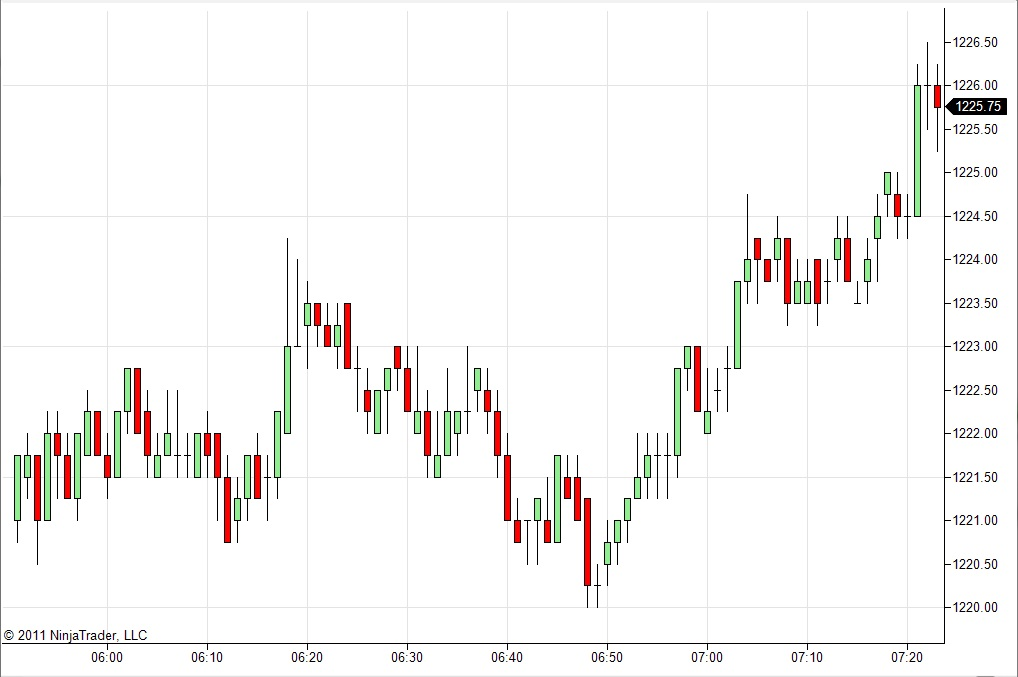
\includegraphics[width=.33\linewidth]{ohlc}}
    \end{figure}
\end{itemize}
\end{frame}

\begin{frame}{Strategie di investimento}
\begin{itemize}
    \item Generalmente occorre comprare quando il titolo ha prezzo basso e vendere quando è alto: \textit{buy} nelle valli e \textit{sell} nei picchi. 
    \item L'operazione va effettuata su base giornaliera / settimanale (breve periodo) e ripetuta spesso
    \item È difficile prevedere il preciso andamento
    \item Se si rileva che il mercato è in forte crescita senza eccessive perdite si può optare per BUY-HOLD: si compra all'inizio e si mantiene il titolo fino alla fine.
    \item Se il mercato crolla, BUY-HOLD segue di conseguenza
    \begin{figure}
    \subfigure{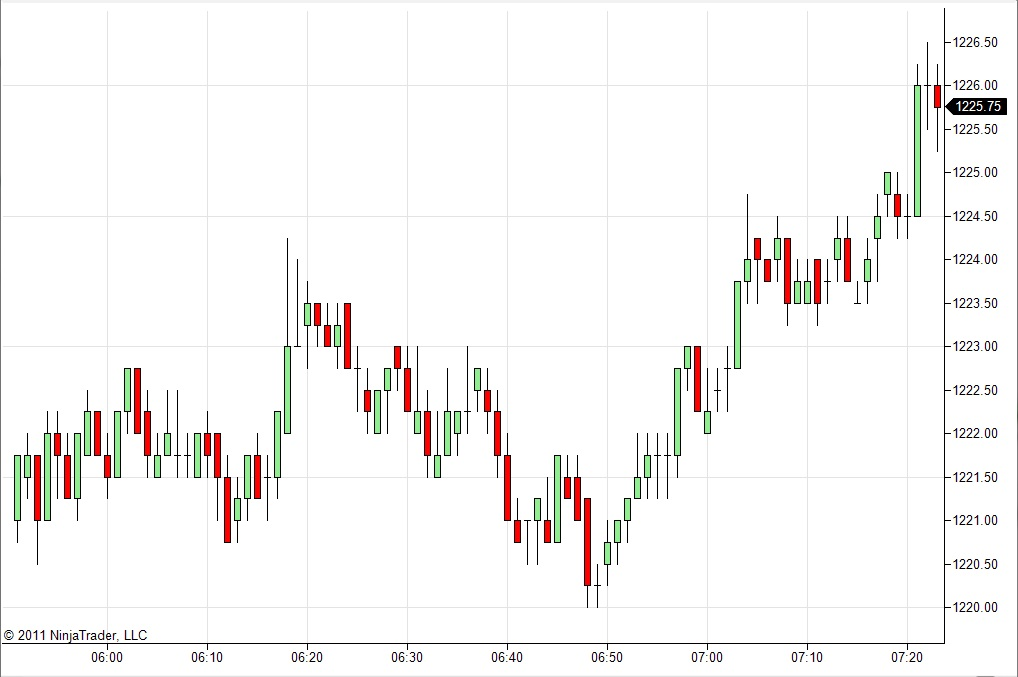
\includegraphics[width=.33\linewidth]{ohlc}}
    \end{figure}
\end{itemize}
\end{frame}

\begin{frame}{Strategie di investimento}
\framesubtitle{Strategie più complesse per il breve termine}
\begin{itemize}
    \begin{block}{SMA}
    Simple Moving Average. Strategia che segnala i cambi di tendenza grazie a due medie mobili, una breve (5 / 10 giorni) e una lenta (100 / 200). Le linee delle medie sono tracciate sul grafico dei prezzi e, quando avviene un'intersezione fra le due, si genera un segnale di \textit{buy} o \textit{sell}.\\ Quando la media breve supera quella lenta il segnale è \textit{buy}. Se la media lenta supera quella veloce si ha la situazione opposta e un segnale di \textit{sell}
    \end{block}
    \begin{figure}
        \centering
        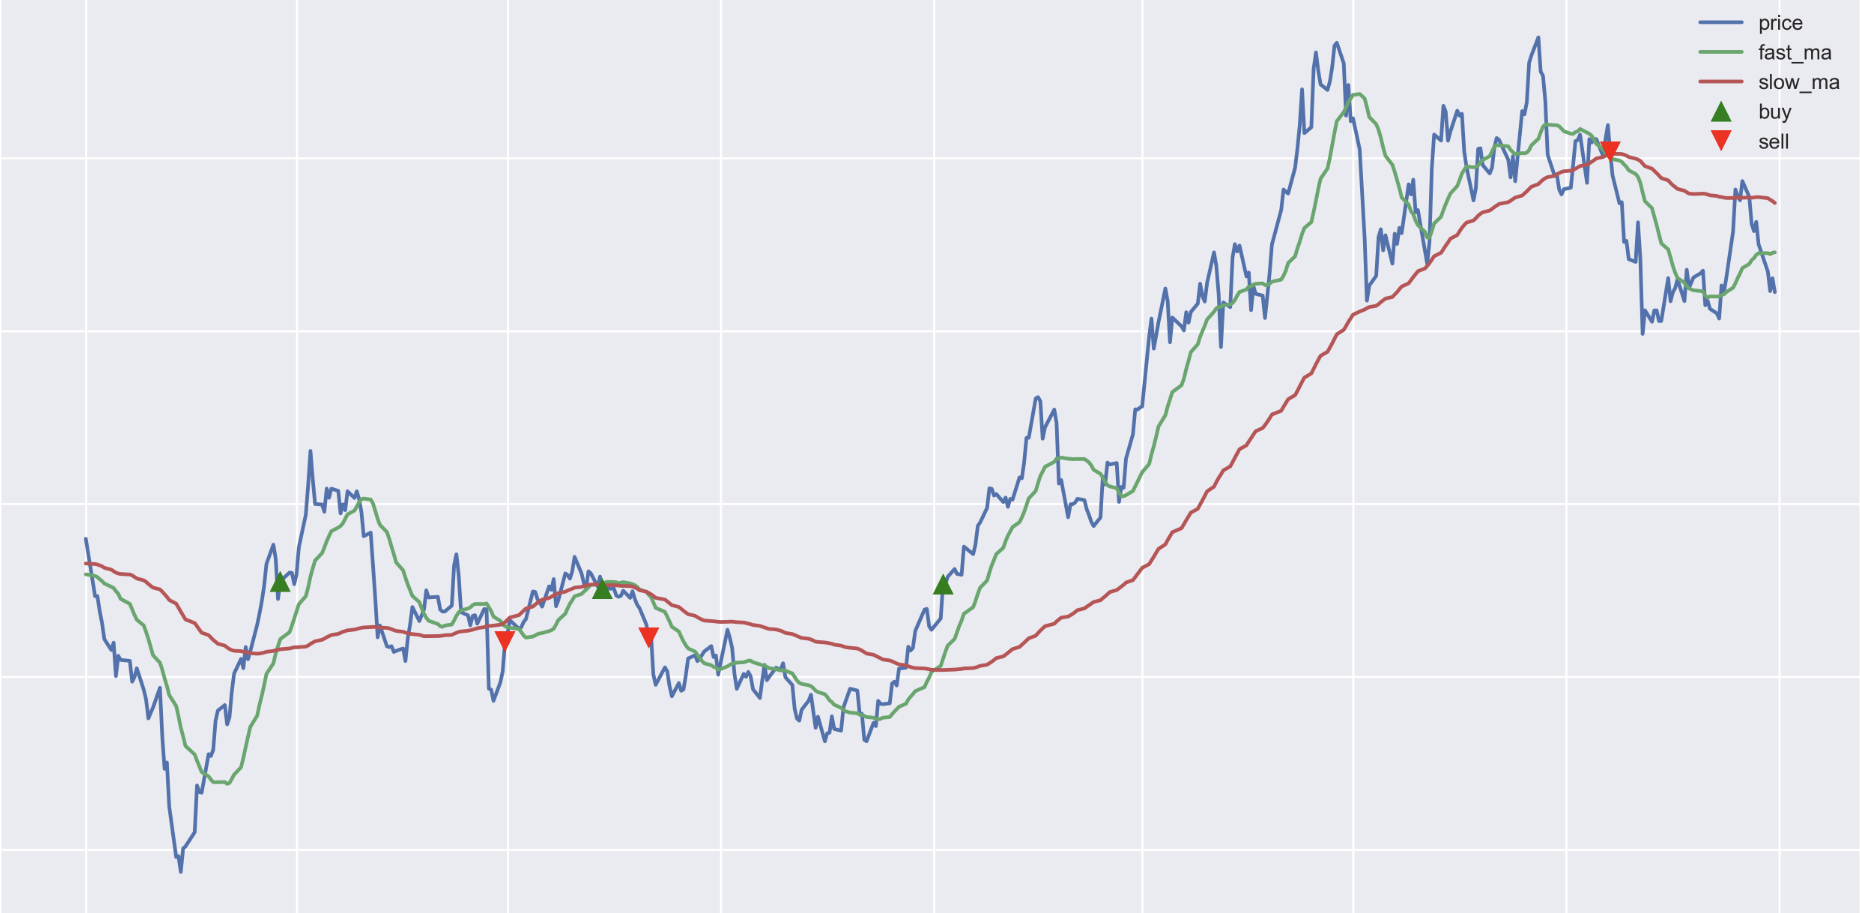
\includegraphics[width=.5\linewidth]{moving_avg2}
    \end{figure}
\end{itemize}
\end{frame}

\begin{frame}{Scopo della tesi}
\begin{itemize}
\item Sentyment AI sceglie quale strategia applicare a seconda della situazione,
dell'andamento dei prezzi e del valore degli indcatori. Per noi è una \textit{black box}
\item L'obiettivo è sviluppare uno strumento in grado di stabilire, a intervalli di tempo definiti,
quale sia la AI migliore all'interno di ogni criptovaluta: \textit{meta-learner}
\item Stabilita la migliore, la si può etichettare come "attiva" ed usare in produzione, permettendogli di piazzare direttamente ordini di acquisto e vendita sul mercato.
\end{itemize}
\end{frame}

\begin{frame}{Scelta della migliore AI}
\framesubtitle{\textit{Meta-learner} e \textit{multi-armed bandit}}
\begin{itemize}
\item \textit{Meta-learner} è basato su \textit{multi-armed bandit}, algoritmo di \textit{reinforcement learning}
\item Si allena sulle performance passate di ciascuna AI
\item Parte da inizio dataset e si sposta a step di 250 record. Poi esplora le AI concorrenti e calcola per ciascuna \textit{guadagno} e \textit{profitto}
\item A ogni step effettua una scelta: decide se scegliere la AI che finora è stata migliore o se esplorarne una nuova, che potrebbe essere anche meglio
\end{itemize}
\begin{figure}
        \centering
        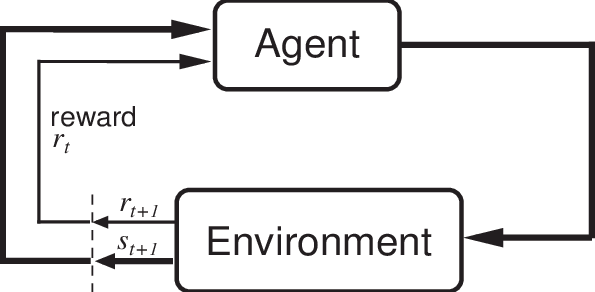
\includegraphics[width=.45\linewidth]{rl}
    \end{figure}
\end{frame}

\begin{frame}{\textit{Meta-learner}}
\begin{itemize}
\item Continuando a registrare le scelte fatte nei vari step, emerge un bandit scelto più spesso di tutti gli altri
\item Dopo un sufficiente numero di step è in grado di dire qual è stata la AI che ha ottenuto performance migliori lungo l'esplorazione
\item Lo stesso algoritmo sarà applicato all'insieme di AI per ciascuna criptovaluta
\item Purtoppo la scarsità di dati non permette iterazioni costanti settimanali o mensili. La scelta è effettuata una sola volta
\end{itemize}
\begin{figure}
        \centering
        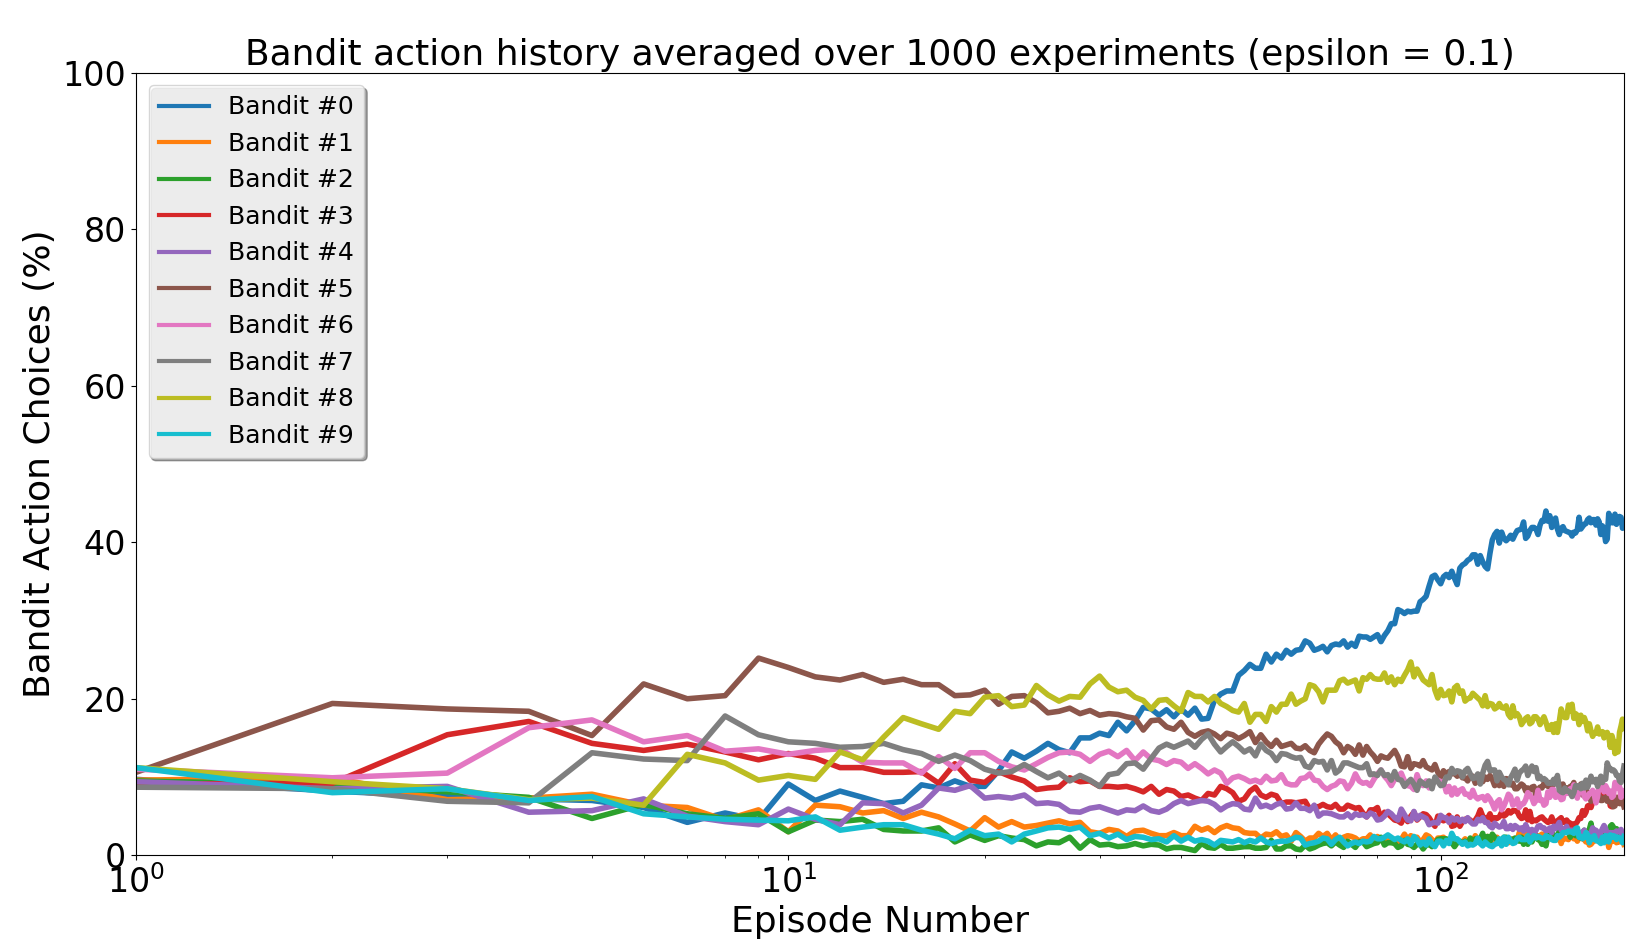
\includegraphics[width=.5\linewidth]{bandit_choice_1000}
\end{figure}
\end{frame}

\begin{frame}{Confronto con altri strumenti}
\begin{itemize}
\item Si rapportano i risultati di Sentyment a strategie di investimento comunemente utilizzate in analisi tecnica (BUY-HOLD, MACD, RSI)
\item Altri strumenti intelligenti di investimento sono proprietari e difficilmente accessibili
\item Diverse metriche di confronto
\begin{itemize}
\item Guadagno assoluto / finale
\item Rendimento (rapporto guadagni - perdite)
\end{itemize}
\item Sentyment pone di più l'attenzione sul limitare le perdite
\item Analizzate le performance lungo tutto il dataset, a finestre di 100 ore. Sul breve periodo Sentyment lavora meglio
\item Generalmente Sentyment è comparabile a altre strategie. Nelle salite è restia a rischiare, nelle discese riesce invece a perdere meno di altri  
\end{itemize}
\end{frame}

\begin{frame}{Confronto con altri strumenti}
\framesubtitle{\textit{Maximum profit}}
\begin{itemize}
\item Modello ottimale di scelte nel breve periodo, costruito a posteriori
\item Approssimato da Genetic Algorithm a causa dell'alta complessità
\item Usato per stabilire un \textit{upper bound}. In genere nessuna strategia si avvicina ai suoi risultati
\item Utile per capire se la differenza di performance fra due strategie è minima o sostanziale
\end{itemize}
\begin{figure}
        \centering
        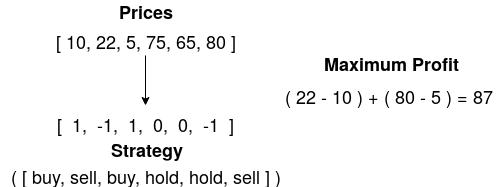
\includegraphics[width=.5\linewidth]{maxprof}
\end{figure}
\end{frame}


\begin{frame}{Risultati e sviluppi futuri}
\begin{itemize}
    \item \textit{Meta-learner} riesce sempre a scegliere la AI che sembra migliore, analizzando il grafico
    \item Il confronto di Sentyment con altri strumenti mostra buoni risultati ed espone punti di forza e debolezze
    \item In futuro 
    \begin{itemize}
        \item Aggiungere un ulteriore livello di learning che sceglie la migliore AI più spesso, cambiando ogni mese sfruttando i brevi picchi di performance
        \item Applicare \textit{meta-learner} a molte più criptovalute
        \item Testare altre AI più simili a Sentyment anche rispetto a \textit{maximum profit}
    \end{itemize}
\end{itemize}
\end{frame}

\end{document}